\documentclass[11pt,twoside,a4paper]{article}
\title{Maths Notes for 2022 Exam}
% Open Sans font for the whole document
\usepackage[default]{opensans}
\usepackage[T1]{fontenc}
\usepackage[a4paper, margin=1.91cm, top=2.91cm, bottom=2.91cm]{geometry}
\usepackage[utf8]{inputenc}
\usepackage{pdfpages}
\usepackage{endnotes}
\usepackage{lipsum}
% Maths symbols and packages
\usepackage{amsmath}
\usepackage{amssymb}
\usepackage{fancyhdr}
\usepackage{multicol}
\pagestyle{fancy}
\fancyhf{}
\setlength{\headheight}{15.2pt}
\fancyhead[LE,RO]{ NEA Analysis }
\fancyfoot[LE,RO]{ \thepage }
\fancyfoot[RE,LO]{ \textit{Max Bowman 2021} }
\usepackage{mdframed}
\newmdtheoremenv[linewidth = 1pt]{theorem}{Theorem}
\usepackage{refcount}
\newcommand{\pagedifference}[2]{%
  \number\numexpr\getpagerefnumber{#2}-\getpagerefnumber{#1}\relax}
%stuff for graphs etc
\usepackage{tikz}
\usepackage{tkz-euclide}
\usepackage{pgfplots}
\pgfplotsset{compat=1.17}
% Add diagrams and images support
\usepackage{graphicx}
\usepackage{microtype}
\graphicspath{ {./images/} {../images/}}
\usepackage{caption}
\usepackage[colorlinks=true,linkcolor=black,urlcolor=blue,bookmarksopen=true]{hyperref}
\usepackage[open,openlevel=1]{bookmark}
\usepackage{mathtools}
\DeclarePairedDelimiter\abs{\lvert}{\rvert}%
\DeclarePairedDelimiter\norm{\lVert}{\rVert}%

% Swap the definition of \abs* and \norm*, so that \abs
% and \norm resizes the size of the brackets, and the 
% starred version does not.
\makeatletter
\let\oldabs\abs
\def\abs{\@ifstar{\oldabs}{\oldabs*}}
%
\let\oldnorm\norm
\def\norm{\@ifstar{\oldnorm}{\oldnorm*}}
\makeatother
\usepackage{subfiles} % Best loaded last in the preamble
\begin{document}
\begin{center}

\thispagestyle{empty}

\vspace*{100pt}

\textbf{\Huge{NEA Analysis}}

\vspace{40pt}

\textbf{\huge{Safe Route Finder for London}}

\vspace{60pt}

{\small \textit{Last updated \today}}

{\small \textit{Pages: \pagedifference{start}{end}}}

\end{center}
\newpage
{
% restrict contents to chapters, sections and subsections
\setcounter{tocdepth}{2}
\tableofcontents
}
\label{start}
\newpage
\section{Problem Area}
There exist a plethora of route finding services for finding the shortest route between two points. These typically optimise for the shortest time taken to travel between two points. Provision for cyclists is however lacking, because it typically consists of an alteration to the existing code for cars, slightly modified to allow for cycle paths and different timings for cyclists.\\
\begin{figure}[t]
    \begin{center}
        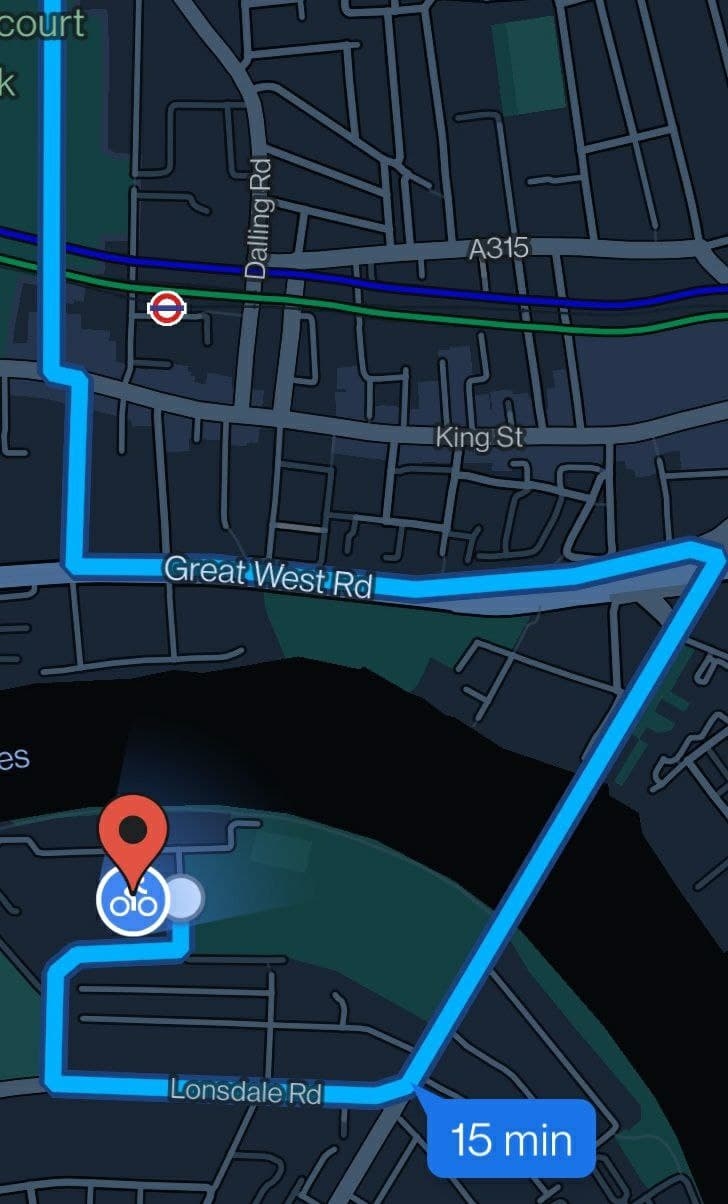
\includegraphics[height=5cm]{route.jpg}
    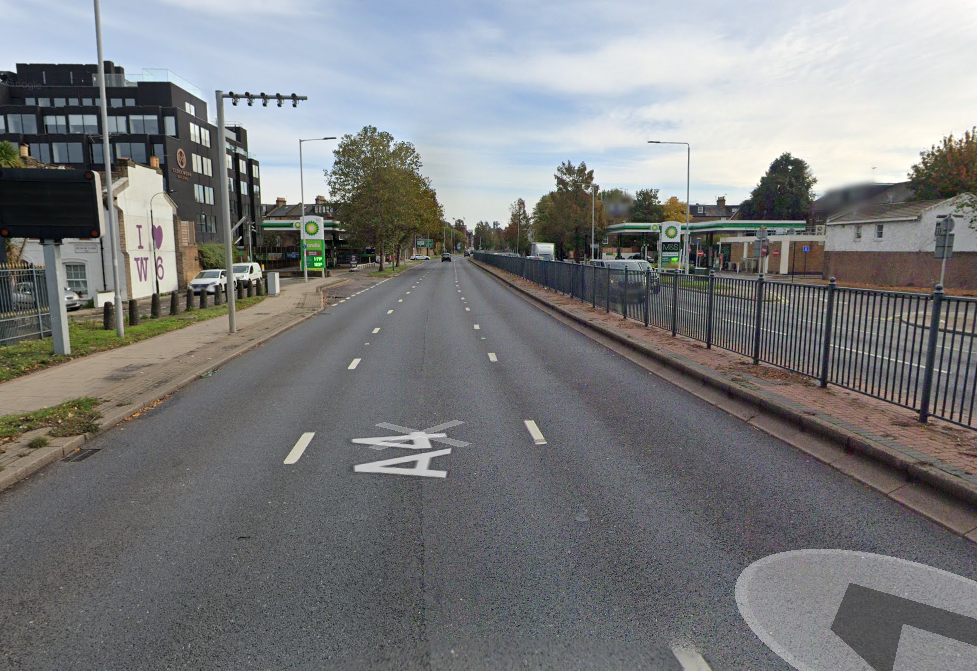
\includegraphics[height=5cm]{dangerous.png}
\end{center}
    \caption{Route suggested by google maps}
    \label{route}
\end{figure}
However many of these route finding applications don't take into account safety. This is shown in Figure \ref{route} which shows the route Google Maps suggests that I cycle to school by. The route includes the A4, which is a very dangerous stretch of road for cyclists as it is a 3 lane road. 
My plan is to combine accident statistics with traffic data to work out which roads are dangerous and then avoid them. 
\section{Problem Solutions}
\label{end}
\end{document}
